\documentclass[tikz,border=10pt]{standalone}
\usepackage{tikz}
\usepackage{amsmath}
\usetikzlibrary{positioning,calc,shapes.arrows,shapes.geometric,decorations.pathreplacing}

\definecolor{errorcolor}{RGB}{231, 76, 60}
\definecolor{gradcolor}{RGB}{155, 89, 182}
\definecolor{updatecolor}{RGB}{46, 204, 113}

\pagecolor{white}

\begin{document}
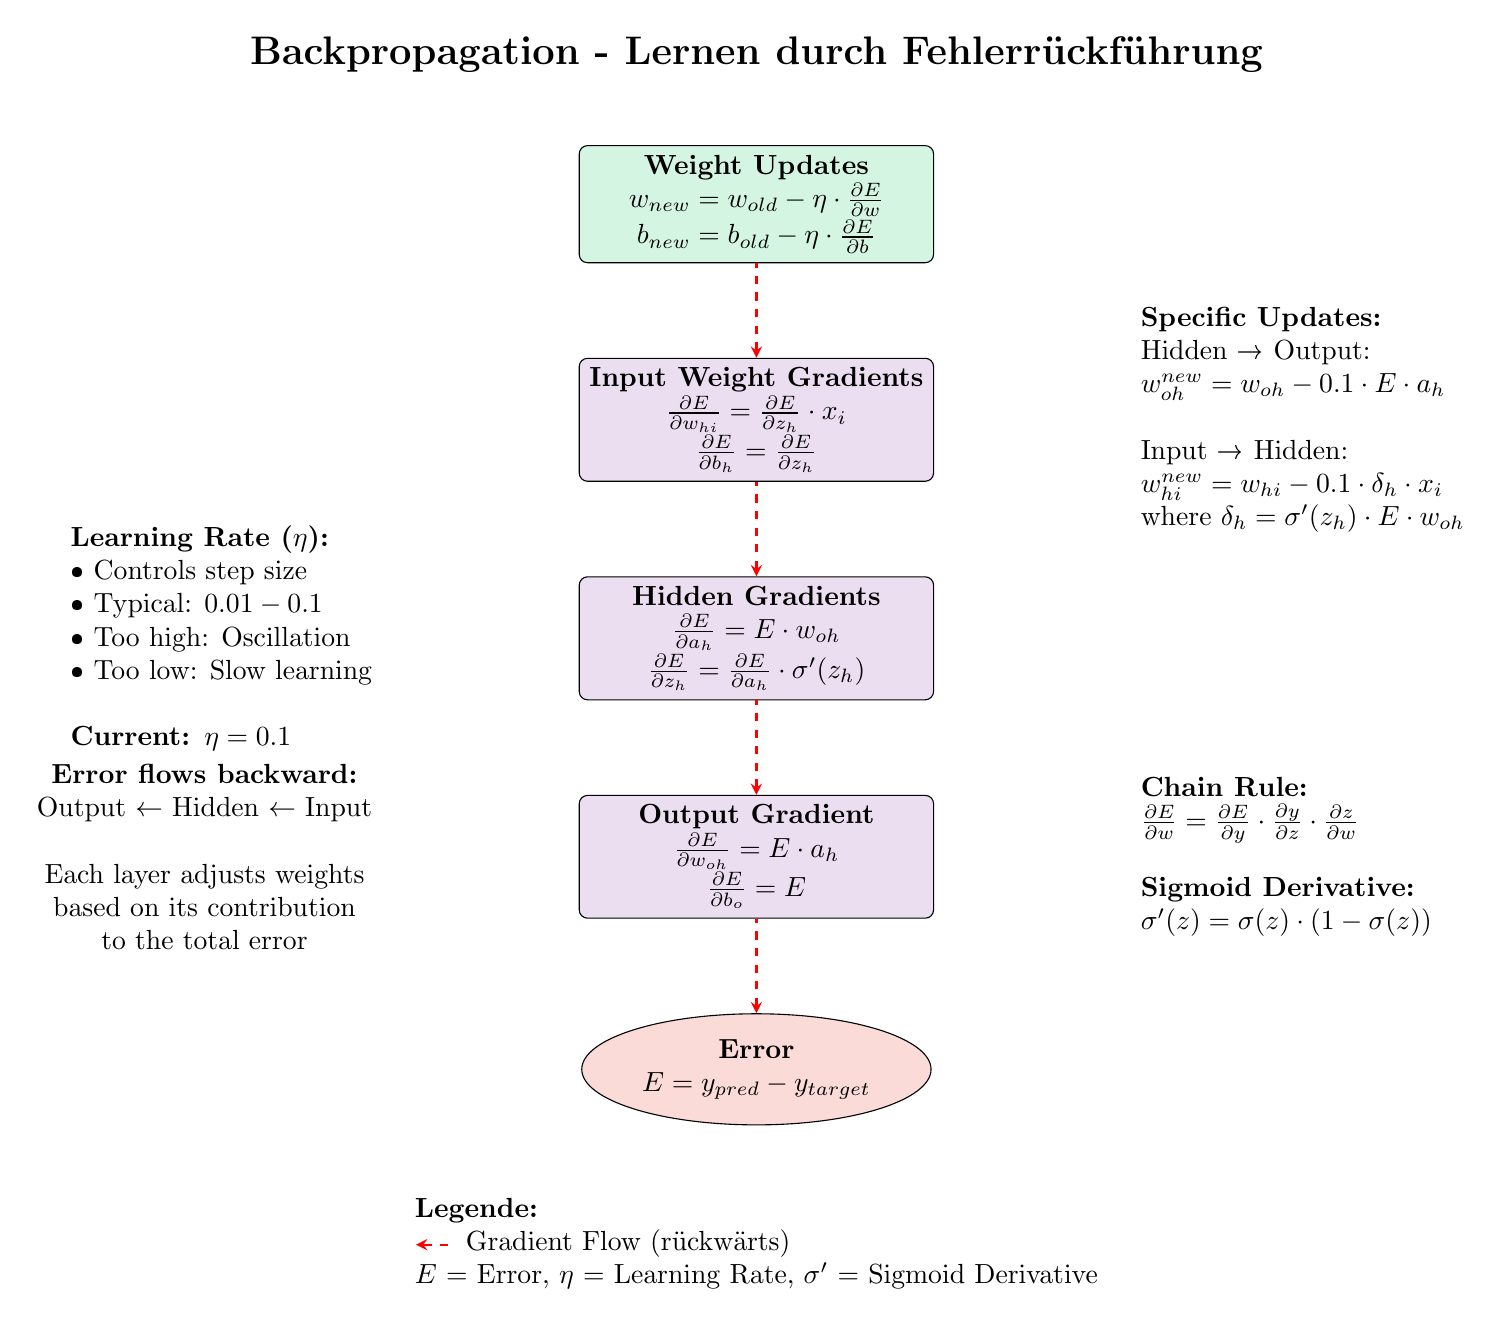
\begin{tikzpicture}[
    node distance=12mm,
    process/.style={rectangle, draw, rounded corners=3pt, minimum width=45mm, minimum height=10mm, align=center},
    data/.style={ellipse, draw, minimum width=30mm, minimum height=8mm, align=center},
    arrow/.style={->, >=stealth, thick},
    backarrow/.style={<-, >=stealth, thick, dashed, red}
]

% Backpropagation Flow (bottom to top)
\node[data, fill=errorcolor!20] (error) {\textbf{Error}\\$E = y_{pred} - y_{target}$};

\node[process, fill=gradcolor!20, above=of error] (output_grad) {
    \textbf{Output Gradient}\\
    $\frac{\partial E}{\partial w_{oh}} = E \cdot a_h$\\
    $\frac{\partial E}{\partial b_o} = E$
};

\node[process, fill=gradcolor!20, above=of output_grad] (hidden_grad) {
    \textbf{Hidden Gradients}\\
    $\frac{\partial E}{\partial a_h} = E \cdot w_{oh}$\\
    $\frac{\partial E}{\partial z_h} = \frac{\partial E}{\partial a_h} \cdot \sigma'(z_h)$
};

\node[process, fill=gradcolor!20, above=of hidden_grad] (input_grad) {
    \textbf{Input Weight Gradients}\\
    $\frac{\partial E}{\partial w_{hi}} = \frac{\partial E}{\partial z_h} \cdot x_i$\\
    $\frac{\partial E}{\partial b_h} = \frac{\partial E}{\partial z_h}$
};

\node[process, fill=updatecolor!20, above=of input_grad] (update) {
    \textbf{Weight Updates}\\
    $w_{new} = w_{old} - \eta \cdot \frac{\partial E}{\partial w}$\\
    $b_{new} = b_{old} - \eta \cdot \frac{\partial E}{\partial b}$
};

% Arrows (backpropagation direction)
\draw[backarrow] (error) -- (output_grad);
\draw[backarrow] (output_grad) -- (hidden_grad);
\draw[backarrow] (hidden_grad) -- (input_grad);
\draw[backarrow] (input_grad) -- (update);

% Side annotations
\node[right=25mm of output_grad, align=left] (chain_rule) {
    \textbf{Chain Rule:}\\
    $\frac{\partial E}{\partial w} = \frac{\partial E}{\partial y} \cdot \frac{\partial y}{\partial z} \cdot \frac{\partial z}{\partial w}$\\
    \\
    \textbf{Sigmoid Derivative:}\\
    $\sigma'(z) = \sigma(z) \cdot (1 - \sigma(z))$
};

\node[left=25mm of hidden_grad, align=left] (learning_rate) {
    \textbf{Learning Rate ($\eta$):}\\
    • Controls step size\\
    • Typical: $0.01 - 0.1$\\
    • Too high: Oscillation\\
    • Too low: Slow learning\\
    \\
    \textbf{Current: $\eta = 0.1$}
};

% Mathematical details for specific updates
\node[right=25mm of input_grad, align=left] (update_details) {
    \textbf{Specific Updates:}\\
    Hidden → Output:\\
    $w_{oh}^{new} = w_{oh} - 0.1 \cdot E \cdot a_h$\\
    \\
    Input → Hidden:\\
    $w_{hi}^{new} = w_{hi} - 0.1 \cdot \delta_h \cdot x_i$\\
    where $\delta_h = \sigma'(z_h) \cdot E \cdot w_{oh}$
};

% Error propagation visualization
\node[left=25mm of output_grad, align=center] (error_flow) {
    \textbf{Error flows backward:}\\
    Output $\leftarrow$ Hidden $\leftarrow$ Input\\
    \\
    Each layer adjusts weights\\
    based on its contribution\\
    to the total error
};

% Title
\node[above=8mm of update, font=\Large\bfseries] {Backpropagation - Lernen durch Fehlerrückführung};

% Legend
\node[below=8mm of error, align=left] {
    \textbf{Legende:}\\
    \tikz[baseline=-0.5ex]{\draw[backarrow] (0,0) -- (0.5,0);} Gradient Flow (rückwärts)\\
    $E$ = Error, $\eta$ = Learning Rate, $\sigma'$ = Sigmoid Derivative
};

\end{tikzpicture}
\end{document}
